\begin{comment}
    

\documentclass[lang=cn,10pt,green]{elegantbook} 
\title{2025年数理经济学笔记}
\subtitle{授课: 杨佳楠老师}

\author{徐靖}
\institute{PKU}
\date{Febuary 27, 2025}
\bioinfo{声明}{请勿用于个人学习外其他用途!}

\extrainfo{个人笔记, 如有谬误, 欢迎指正! 联系方式 : 2200012917@stu.pku.edu.cn}

\setcounter{tocdepth}{3}
\logo{pkuhub-cn.png}
\cover{cover.jpg}


% 本文档命令
\usepackage{array}
\newcommand{\ccr}[1]{\makecell{{\color{#1}\rule{1cm}{1cm}}}}

% 修改标题页的橙色带
% \definecolor{customcolor}{RGB}{32,178,170}
% \colorlet{coverlinecolor}{customcolor}

\begin{document}

\maketitle
\frontmatter

\tableofcontents

\mainmatter
% \end{comment}
% TODO

\chapter{Multi-Variable Optimization with Inequality
Constraints}

\begin{introduction}[Keywords]
    \item Complementary slackness 互补松弛条件
    \item Karush-Kuhn-Tucker Theorem KKT 条件
    \item Constraints Qualification 约束资格条件
    \item Convex Optimization 凸优化
    \item Nondegenerate Constraint Qualification NDCQ 非退化约束资格条件
    \item Slater Condition SCQ 斯莱特条件
\end{introduction}

\section{Optimization with linear inequality constraints}
\subsection{Geometric intuition for FOC}
考虑一个优化问题:
\begin{align*}
    \min_{x \in \mathbb{R}^n} & \quad f(x) \\
    \text{s.t.} & \quad Ax \leq b \\
    & \quad x \geq 0
\end{align*}
我们的目标是去找到 $x^*$ 作为局部最小的必要条件.
\begin{definition}[Constraint Set]
    \begin{align*}
        \Omega = \{x \in \mathbb{R}^n | Ax \leq b\}
    \end{align*}
    其中 $A$ 是 $m \times n$ 的矩阵, $b$ 是 $m$ 维向量.
\end{definition}

先考虑一条直线作为约束, 即 $a^T x \leq c$.
\begin{itemize}
    \item 如果 $a^T x^* < c$, 那么满足 $\nabla f(x)=0$ 的 $x^*$ 是局部最优
    \item 如果 $a^T x^* = c$, 那么 $x^*$ 是局部最优的充分必要条件是 $\nabla f(x^*)$ 和 $a$ 线性相关.
\end{itemize}

这是因为对任意可行的方向 $d$, 有: 
$$0\leq\lim_{t\to 0}\frac{f(x^*+td)-f(x^*)}{t}=\langle\nabla f(x^*),d\rangle$$

这意味着 $\nabla f(x^*)$ 和 $d$ 线性相关, 实际上 
$$\nabla f(x^*)+\lambda a = 0, \lambda \ge 0$$

\begin{definition}[feasible direction]
    $d$ 是可行的方向, 如果 $x^*+td \in \Omega$ 对任意小的 $t>0$ 都成立.
\end{definition}
考虑两条直线的约束, 对于其交点 $x^*$, 其成为局部最优的直观的必要条件是:
$$\nabla f(x^*)+\lambda_1 a_1 + \lambda_2 a_2 = 0, \lambda_1, \lambda_2 \ge 0$$

\begin{figure}
    \centering
    \begin{minipage}{0.49\textwidth}
        \centering
        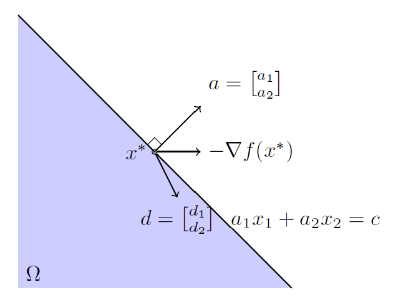
\includegraphics[width=\linewidth]{gradient-1.png}
        \caption{$-\nabla f$只能延 $a$ 的方向}
        \label{fig:gradient-1}
    \end{minipage}\hfill
    \begin{minipage}{0.45\textwidth}
        \centering
        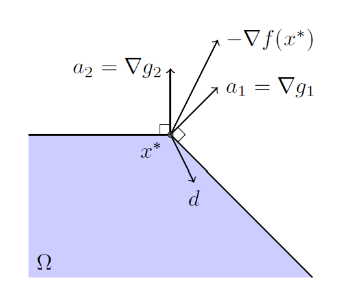
\includegraphics[width=\linewidth]{gradient-2.png}
        \caption{$-\nabla f$可以延 $a_1,a_2$ 所夹任意方向}
        \label{fig:gradient-2}
    \end{minipage}
\end{figure}

\newpage

\subsection{KKT}

因此, 对于线性约束的优化问题, 我们给出一个相对统一严谨的必要条件:
\begin{theorem}[Modified Karush-Kuhn-Tucker Theorem]
对于优化问题:
\begin{align*}
    \min_{x \in \mathbb{R}^n} & \quad f(x) \\
    \text{s.t.} & \quad g_i(x) \leq 0, i\in [I] \\
    & \quad h_j(x) = 0, j\in [J]
\end{align*}
其中, $f$ 可微, $g_i = \langle a_i,x \rangle-c_i$, $h_j = \langle b_j,x \rangle - d_j$ 均为线性函数, $a_i,b_j \neq 0$.
如果 $x^*$ 是局部最优解, 那么存在 $\lambda_i $ 和 $\mu_j$ 使得:
\begin{align*}
    \nabla f(x^*) + \sum_{i=1}^I \lambda_i \nabla g_i(x^*) + \sum_{j=1}^J \mu_j \nabla h_j(x^*) = 0 \\
    \lambda_i \geq 0, g_i(x^*) \leq 0, \lambda_ig_i(x^*) = 0 \\
    h_j(x^*) = 0 \\
\end{align*}
\end{theorem}
\begin{note}
    KTT 条件可以由拉格朗日乘子法得到, 其中三个条件分别对应于: 一阶条件, 互补松弛, 等式约束.
    \end{note}

\section{Optimization with nonlinear inequality constraints}
\subsection{General KKT}
线性约束的优化问题 (线性规划) 是简单的, 非线性是坏的性质. 一个直观的想法是用Taylor展开近似线性约束.
$$g_i(x)\approx g_i(x^*)+\langle\nabla g_i(x^*),x-x^*\rangle$$

\clearpage
因此我们引入一类条件, 统称约束资格条件 constraint qualigication (CQ). 使之代替原本的 g,h 线性条件. (本质是作近似) 然后重写 KTT \footnote{实际上, 课堂所展示的 General KKT 忽略了等式约束的函数组 $h$, CQ 条件也忽略. (从 $g$ 扩充到 $h$ 是显然的, 例如 NDCQ 中 $h$ 自然在 $I(x^*)$ 中, 但 $g$ 不一定在 $I(x^*)$ 中.)}:

\begin{theorem}[General Karush-Kuhn-Tucker Theorem]
    对于优化问题:
    \begin{align*}
        \min_{x \in \mathbb{R}^n} & \quad f(x) \\
        \text{s.t.} & \quad g_i(x) \leq 0, i\in [I] \\
        & \quad h_j(x) = 0, j\in [J]
    \end{align*}
    其中, $f$ 可微, $x^*$ 是局部最优解, \colorbox{yellow}{且约束资格条件 CQ 成立}, 那么存在 $\lambda_i $ 和 $\mu_j$ 使得:
    \begin{align*}
        \nabla f(x^*) + \sum_{i=1}^I \lambda_i \nabla g_i(x^*) + \sum_{j=1}^J \mu_j \nabla h_j(x^*) = 0 \\
        \lambda_i \geq 0, g_i(x^*) \leq 0, \lambda_ig_i(x^*) = 0 \\
        h_j(x^*) = 0 \\
    \end{align*}
    \end{theorem}

\subsection{Constraint Qualification}
课堂上给出了两种:
\begin{definition}[Nondegenerate CQ (NDCQ)]
    令 $I(x^*)$ 为 $x^*$ 积极约束的指标集 (set of active constraint indices), 即 
    $$ I(x^*) = \{i | g_i(x^*) = 0\} $$
    NDCQ : 活跃约束的梯度线性无关, 即:
    $$\text{rank} \left( \nabla g_i(x^*), i \in I(x^*) \right) = |I(x^*)|$$
\end{definition}
\note{线性无关的意义在于, 保证了 $\lambda$ 的唯一性. 且确保 $\nabla f$ 一定在这些梯度张成的空间. 几何上可以理解为, 可行方向(f的梯度方向)和起作用的/活跃的约束梯度方向正交}
\begin{definition}[Slater Condition(SCQ)]
    \begin{itemize}
        \item $g_i'$ 是凸的
        \item 存在 $x_0$ 使得 $g_i(x_0) < 0, i \in [I]$, 即 $x_0$ 是严格可行的 (strictly feasible).
    \end{itemize}
\end{definition}

\section{Convex Optimization}
应用到凸优化问题上, 我们可以得到更强的结论.
\begin{definition}[Convex Optimization (无等式约束版)]
    \begin{align*}
        \min_{x \in \mathbb{R}^n} & \quad f(x) \\
        \text{s.t.} & \quad g_i(x) \leq 0, i\in [I] 
    \end{align*}
    其中 $f, g'_i$ 可微且凸. 
\end{definition}
\begin{proposition}
    \textbf{Necessity} : 如果 $x^*$ 是局部最优解, 且存在 $x_0$ 使得 $g_i(x_0) < 0, i \in [I]$, 那么存在拉格朗日乘子 $\lambda_i$ 使得 KKT 条件成立.

    \textbf{Sufficiency} : 如果存在拉格朗日乘子 $\lambda_i$ 使得 KKT 条件成立. 则 $x^*$ 是全局最优解.
\end{proposition}
\note{必要性即以 SCQ 为假设的 KTT. 充分性证明不难: $x^*$ 最小化 $L(x,\lambda)$, 从而对任意可行的 $x$, 有$f(x^*) =  L(x^*,\lambda) \leq L(x,\lambda) \leq f(x)$.}

理论成立, 做题可以三步走:
\begin{enumerate}
    \item Verify Condition
    \begin{itemize}
        \item $f,g'_i$ 可微且凸吗
        \item SCQ 成立吗
    \end{itemize}
    \item Form Lagrangian $L(x,\lambda)$
    \begin{itemize}
        \item First-order condition
        \item Complementary slackness
    \end{itemize}
    \item Solve System
    \begin{itemize}
        \item Solve for $x^*, \lambda^*$
        \item $x^*$ 是原问题解, $\lambda^*$ 提供灵敏度信息
    \end{itemize}
\end{enumerate}
%\end{document}







